% Nejprve uvedeme tridu dokumentu s volbami
\documentclass[english,master,public,dept460,male,cpdeclaration,oneside]{diploma}
% Dalsi doplnujici baliky maker
%\usepackage[english]{babel}
\usepackage{subfig}		% makra pro "podobrazky" a "podtabulky"
\usepackage{tikz}		% makra pro kresleni


% Zadame pozadovane vstupy pro generovani titulnich stran.
\ThesisAuthor{Bc. Ľubomír Sokolovský}

\EnglishThesisTitle{Multiplatform Mobile Application Development Methodology}

\CzechThesisTitle{Metodika vývoje multiplatformní mobilní aplikace}

\SubmissionDate{28th April 2017}

% Pokud nechceme nikomu dekovat makro zapoznamkujeme.
\Thanks{Rád bych na tomto místě poděkoval všem, kteří mi s prací pomohli, protože bez nich by tato práce nevznikla.}

% Zadame cestu a jmeno souboru ci nekolika souboru s digitalizovanou podobou zadani prace.
% Pokud toto makro zapoznamkujeme sazi se stranka s upozornenim.
\ThesisAssignmentImagePath{Figures/Assignment}

% Zadame soubor s digitalizovanou podobou prohlaseni autora zaverecne prace.
% Pokud toto makro zapoznamkujeme sazi se cisty text prohlaseni.
\AuthorDeclarationImageFile{Figures/AuthorDeclaration.jpg}

% Zadame soubor s digitalizovanou podobou souhlasu spolupracujici prav. nebo fyz. osoby.
% Pokud toto makro zapoznamkujeme sazi se cisty text souhlasu.
\CooperatingPersonsDeclarationImageFile{Figures/CoopPersonDeclaration.jpg}

\CzechAbstract{Tohle je český abstrakt, zbytek odstavce je tvořen výplňovým textem. Naší si rozmachu potřebami s posílat v poskytnout ty má plot. Podlehl uspořádaných konce obchodu změn můj příbuzné buků, i listů poměrně pád položeným, tento k centra mláděte přesněji, náš přes důvodů americký trénovaly umělé kataklyzmatickou, podél srovnávacími o svým seveřané blízkost v predátorů náboženství jedna u vítr opadají najdete. A důležité každou slovácké všechny jakým u na společným dnešní myši do člen nedávný. Zjistí hází vymíráním výborná.}

\CzechKeywords{typografie, \LaTeX, diplomová práce}

\EnglishAbstract{This is English abstract. Lorem ipsum dolor sit amet, consectetuer adipiscing elit. Fusce tellus odio, dapibus id fermentum quis, suscipit id erat. Aenean placerat. Vivamus ac leo pretium faucibus. Duis risus. Fusce consectetuer risus a nunc. Duis ante orci, molestie vitae vehicula venenatis, tincidunt ac pede. Aliquam erat volutpat. Donec vitae arcu. Nullam lectus justo, vulputate eget mollis sed, tempor sed magna. Curabitur ligula sapien, pulvinar a vestibulum quis, facilisis vel sapien. Vestibulum fermentum tortor id mi. Etiam bibendum elit eget erat. Pellentesque pretium lectus id turpis. Nulla quis diam.}

\EnglishKeywords{typography, \LaTeX, master thesis}

\AddAcronym{DVD}{Digital Versatile Disc}
\AddAcronym{TNT}{Trinitrotoluen}
\AddAcronym{UML}{Unified Modeling Language}
\AddAcronym{HTML}{Hyper Text Markup Language}
\AddAcronym{TUG}{\TeX{} Users Group}


% Zacatek dokumentu
\begin{document}

% Nechame vysazet titulni strany.
\MakeTitlePages

% Pokud mame v zaverecne praci vypisy kodu, jinak odstranit.
\lstlistoflistings

\section{Introduction}
Competition is a natural trait of any market. It offers customers with the possibility to choose between multiple variants. At the same time, it forces the producers to innovate and outweigh disadvantages of their products with bonus features. 

Just like any other market, this is true also for smartphones and mobile operating systems. However, the benefits and variety for customers on one hand represent challenges for mobile app developers on the other. They stand before a difficult decision - to either implement their application multiple times for each operating system, or stay exclusive to a single platform and ignore all the others.

Another problem, besides the fragmentation, are the perpetual changes in operating systems themselves and their market shares. While only few years ago, Symbian was the dominant platform, since 2010 Android is the king of the smartphone world. Between years 2009-2016 there have been 12 major version changes and 24 API changes for Android. It is similar for iOS, currently the second strongest mobile OS, with 10 different versions since 2008. While Android and iOS changed their versions, they remained faithful to their respective development technologies. This cannot be said of Windows, which from Windows Phone 7 to Windows 10 Mobile swapped several different technologies (XNA, WinRT, Silverlight and UWP).

Implementing the same app over and over again using different languages and APIs is a boring and tedious task for developers, and a waste of time and money for IT companies. Soon, solutions and tools allowing development for multiple platforms, while writing the code just once, began to emerge. As of September 2016, there can be found more than 100 of these multi-platform development tools for mobile operating systems.

Some of these tools offer code-free programming. Others provider optimization of web applications for mobile browsers. There are solutions for truly native apps developed with a single code base, or hybrid apps that are programmed as web apps, but have access to device hardware. And for game developers, there are multiple frameworks and engines for both 2D and 3D development. 

However, choosing the right development tool can be a difficult task. Often, many products seem to provide the same functionality. The devil is always in the details, and discovering a missing framework capability in the middle of development process can result in wasting of several months of work. The purpose of this thesis is to create a methodology, that will guide the developers, architects and managers and help them to find the most suitable development tools, that will fulfill all their criteria.

\subsection{Thesis overview}
Because there are so many different multi-platform development solutions and not all of them can be covered, we will make the target group a little narrower. In the first chapters, this thesis will try to determine which operating systems are still relevant for the multi-platform development. We will analyze the global mobile operating systems market, smartphone sales, application revenues and developers’ focus. 

After that we will take the relevant operating systems and focus only on multi-platform development tools which enable creating apps for the most used OSs. Since we want to focus on the possibility of using device hardware and native API, we will ignore all web-based solutions and game engines. The thesis will omit also all tools which do not enable general development options (e.g. tools focused only on a single company or activity).

From the products which passed the filter, we will pick a few ones and test their usability on a couple of pre-defined use cases. The thesis will discuss and compare the implementation details, strengths, weaknesses and limitations of individual development tools. The results of these implementations, as well as theoretical research, will be helpful in establishing a set of factors crucial in the creation of the resulting methodology.

The methodology itself will consist of several parts. The first part will validate projects and requirements, to which the methodology is relevant. The second part will be the core of the methodology, helping the user determine the right multi-platform development tool. The last part will contain suggestions for additional research which can be performed by the user if the methodological results were indefinite.

\subsection{Remarks}
The reader may be familiar with the term “cross-platform” development. This term is interchangeable with “multi-platform” \footnote{https://en.wikipedia.org/wiki/Cross-platform}, which is used in this thesis. Both cross-platform and multi-platform software development refer to the process of creating a piece of software that can be run on multiple platforms.

Considering the Windows operating system, Microsoft had several products for mobile devices. From 2000 to 2010 they delivered several versions of the Windows Mobile product line. It was succeeded by Windows Phone 7, 8 and 8.1. In 2015, Microsoft introduced their Windows 10 operating system with common core for desktop, tablet, smartphone and IoT development \footnote{https://developer.microsoft.com/en-us/windows}. The version for smartphones is called Windows 10 Mobile \footnote{https://en.wikipedia.org/wiki/Windows\_10\_Mobile}, similar to the old product line from the previous decade, although being an iteration of Windows Phone 8.1. To avoid long and confusing names and distinguish the mobile and desktop versions, we will call the Microsoft operating system for smartphones simply Windows. In a more narrow context, under Windows we will understand Windows 10 Mobile and the previous version, Windows Phone 8.1, which has forward-compatible applications \footnote{https://blogs.windows.com/buildingapps/2014/12/17/bring-your-windows-phone-silverlight-apps-to-windows-runtime-xaml-prepare-for-universal-app-development-in-windows-10/}. 
Regarding tables and charts, if not stated otherwise, the data are presented for the year 2016.



\section{Relevant mobile operating systems}
In order to create a methodology for choosing the right mobile multi-platform development tool we first need to specify which platforms will be targeted. Throughout the time there have been many more or less successful mobile operating systems. The trend shifts in mobile market are one of the most dynamic compared to other market types. This is caused mainly by two following factors:
\begin{enumerate}
	\item The mobile market is very young. Mobile phones became commercially available to the wide public only about 30 years ago, in the late 1980s and early 1990s. 
	\item They became increasingly popular, making them an interesting technology for development and investing, offering high profit. 
\end{enumerate}


By the end of millennium, mobile phones were almost in every family in the western hemisphere \footnote{http://data.worldbank.org/indicator/IT.CEL.SETS.P2?view=map\&year=2000}. However, they were still used mainly for telephony and sending SMS, with occasional MMS in the first years of 2000s. There were only few devices, which tried to combine mobile phones with PDAs - small personal computers, targeted mainly for business and enterprise environments. They were running on operating systems such as Palm OS, BlackBerry OS and Windows CE, which later evolved into smartphone operating systems.

These hybrids of mobile phones and PDAs were the first predecessors of today’s smartphones. Probably, the most known series are Nokia 9000 Communicator devices. In 2000, Ericsson released E380, which was the first device marketed as “smartphone”. It was also the first device running Symbian OS, the dominant mobile operating system until 2010.

Several other companies have seen the potential of these hybrid devices, which combined mobility, telephony, computing power and allowed connection to the ever-growing Internet. Soon, Symbian, Palm, BlackBerry and Windows Mobile got new rivals. It was iOS in 2007, Android in 2008 and Bada in 2009. These new players shattered the mobile market - and two of them even surpassed the old operating systems. 

Today, the situation is very different than it was ten years ago. Symbian OS, Palm OS and Bada are all discontinued projects. BlackBerry OS (known as RIM) is at the brink of existence. Windows Mobile was replaced by Windows Phone, but has lost a large portion of the market. The dominant roles are held by iOS and Android.

\begin{figure}
	\centering\includegraphics[width=0.8\textwidth]{Figures/World_Wide_Smartphone_Sales_Share.png}
	\caption{World-wide smartphone sales [https://en.wikipedia.org/wiki/Mobile\_operating\_system\#/]}
\end{figure}

\subsection{Current situation}
Specifying, which operating systems are relevant to our methodology is not a trivial task, if we want the methodology to be accurate also for years to come. Yet, there are several factors, which may help us determine the trends to come:
\begin{enumerate}
	\item Is the OS still officially supported?
	\item What is the current market share of active users?
	\item What are the market shares of the sales?
	\item What are the revenues for developing applications for a particular OS?
	\item How many developers support the OS?
\end{enumerate}
Answering these questions will help us assign priority to individual smartphone platforms. 

\subsubsection{Supported operating systems}
As of the August 2016, the following smartphone operating systems are still being developed and supported: 
\begin{itemize}
	\item Android (with multiple modifications, such as Cyanogen, Fire OS or MIUI)
	\item BlackBerry 10 (RIM OS)
	\item Firefox OS
	\item H5OS
	\item iOS
	\item Sailfish OS
	\item Tizen
	\item Ubuntu Touch OS
	\item Windows 10 Mobile (previously Windows Phone 8.1)
\end{itemize}

\subsubsection{Smartphone OS usage market share}
The following table shows the percentage of smartphone users for each smartphone OS (for the year 2016) \footnote{https://www.netmarketshare.com/operating-system-market-share.aspx?qprid=8\&qpcustomd=1}:

\begin{table}
	\centering
	\caption{Smartphone OS usage market share}
	\begin{tabular}{l r r}
		\toprule		
		Platform & Market share (\%) & Devices (approximate, in millions) \\
		\midrule
		Android & 65.33\% & 1371.93 \\
		iOS & 27.8\% & 583.8 \\
		Windows & 2.64\% & 55.44 \\
		BlackBerry & 1.18\% & 24.78 \\
		Symbian & 1.15\% & 24.15\\
		Other & 1.9\% & 39.9\\
		\midrule
	\end{tabular}
\end{table}

The approximate number of active devices is based on the figure that there is about 2.1 billion smartphones in use worldwide \footnote{http://www.statista.com/statistics/330695/number-of-smartphone-users-worldwide/}. With more than a billion active devices, Android is clearly the most used mobile operating system. iOS is also very strong, having more than a quarter of the market share. The other platforms are far behind. Windows users are just a tenth compared to Apple’s iPhone and iPad users. The portion BlackBerry’s RIM users is just slightly above 1\%. Symbian, having a similar share although being discontinued, is still used by more than 20 million users.

\subsubsection{Smartphone OS sales market share}
The smartphone sales market share can help us predict the future growth or decline of a certain platform. As seen in the graph XX earlier in this chapter, there was a dramatic shift in 2010 and 2011, when Android surpassed Symbian in the percentage of sold smartphones.

\begin{table}
	\centering
	\caption{Smartphone OS sales, various reports from http://www.gartner.com/technology/home.jsp}
	\begin{tabular}{l l l l l l l l}
		\toprule
		Year & RIM & Symbian & iOS & Android & Bada & Windows & Other\\
		\midrule		
		2016 & 0.19\% & - & 14.78\% & 84.1\% & - & 0.7\% & 0.23\% \\
		2015 & 0.37\% & - & 16.26\% & 80.52\% & - & 2.47\% & 0.38\% \\
		2014 & 0.6\% & - & 15.4\% & 80.7\% & - & 2.8\% & 0.5\% \\
		2013 & 1.9\% & 0.1\% & 15.6\% & 78.4\% & 0.2\% & 3.2\% & 0.6\% \\
		2012 & 5\% & 4.2\% & 19.1\% & 66.4\% & 2.3\% & 2.5\% & 0.5\% \\
		2011 & 10.9\% & 18.74\% & 18.92\% & 46.53\% & 2.01\% & 1.65\% & 1.21\% \\
		\midrule		
	\end{tabular}
\end{table}

By the end of 2013, Symbian and Bada were pronounced discontinued. Windows Mobile transformed to Windows Phone in 2010. However, the transformation was not very successful. Windows Phone’s sales peaked at 3.2\% in 2013 and have been decreasing ever since. Compared to the 12\% market share of Windows Mobile in 2007, this situation looks very bleak for Microsoft. 

Even worse, however, are the numbers for another former major smartphone OS. BlackBerry’s RIM had almost 20\% market share in 2009. Now, for two years its sales have dropped below 1\%. iOS on the second place has its sales market share fluctuating around 15\%, but there is a large gap between the second and the first place. Android, now with stunning 84.1\% of all smartphone sales is the major force in the industry. 

Yet, the raw sales percentages may not necessarily correspond to the change of user base in absolute numbers. There is the possibility that Android users are buying new devices more often compared to iOS or Windows users, resulting in higher sales. But it definitely shows the trends whether a certain platform is experiencing its rise or fall.

For certain businesses, the global data may not be relevant, since regionally the sales percentages differ substantially.

\begin{table}
	\centering
	\caption{Regional smartphone sales in 2016}
	\begin{tabular}{l l l l l l}
		\toprule
		\% & Android & BlackBerry & iOS & Windows & Other \\
		\midrule
		USA & 58.2 & 0.1 & 39.1 & 2.6 & 0 \\
		Mexico & 90.5 & 0.7 & 5 & 2.6 & 1.2 \\
		Brazil & 92.4 & 0 & 3.3 & 4.1 & 0.1 \\
		Argentina & 83.5 & 3.4 & 0.9 & 9.1 & 3.2 \\
		UK & 52.6 & 0.2 & 38.6 & 8.6 & 0 \\
		Germany & 74.2 & 0.6 & 19.3 & 5.9 & 0.1 \\
		France & 71.8 & 0.5 & 19.3 & 7.8 & 0.5 \\
		Spain & 87.8 & 0 & 11.4 & 0.8 & 0 \\
		Italy & 78.1 & 0.2 & 14.4 & 7.2 & 0.1\\
		Russia & 71.2 & 0.6 & 14.8 & 10.6 & 2.7 \\
		China & 73.9 & 0 & 25 & 0.9 & 0.3 \\
		Japan & 48.7 & 0 & 50.3 & 0.5 & 0.5 \\
		Australia & 52.6 & 0.2 & 41.2 & 5.4 & 0.6 \\
		World & 84.1 & 0.19 & 14.87 & 0.7 & 0.23 \\
		\midrule
	\end{tabular}
\end{table}

\begin{figure}
	\centering\includegraphics[width=0.8\textwidth]{Figures/regionalMarketShares.png}
	\caption{Regional market shares [http://www.kantarworldpanel.com/global/smartphone-os-market-share/intro]}
\end{figure}

\subsubsection{Smartphone app stores revenues}
The sheer numbers of mobile platform users or device sales is one thing. But many developers - and almost all businesses - are motivated by something else entirely. Money may be a very decisive factor in choosing, which platforms will be targeted and which will be omitted. 

For some time now, it is common knowledge that Android users are not as willing to pay for apps as their iOS colleagues \footnote{https://www.macobserver.com/tmo/article/new\_report\_shows\_ios\_users\_spend\_money\_like\_to\_check\_weather}. This has been true also in recent years. Although the number of downloaded apps in Google Play is twice as high compared to Apple’s App Store, iOS is creating 70\% more revenue compared to Android \footnote{http://www.latinpost.com/articles/110519/20160121/ios-vs-android-market-share-revenue-one-win-for-each-app-store-in-2015.htm}. 

These data are backed also by a survey performed by InMobi \footnote{http://www.lifehacker.com.au/2016/03/how-much-do-mobile-developers-make-per-app/}. While on average an Android developer\footnote{The survey does not distinguish between individual developers, developer groups or companies - all three are represented by the term "developer"} makes \$4900 per month, an iOS developer earns \$8100. However, there is a much more interesting discovery made by the survey. Developers targeting Windows earn the most - on average \$11400 per month.

\begin{figure}
	\centering\includegraphics[width=0.8\textwidth]{Figures/appRevenues.png}
	\caption{Average app revenues from individual app stores, per month}
\end{figure}

The article explains this by the small amount of apps found on Windows Store. Smaller market means less competition and this has dual effect on the market. The discoverability factor of your application is much higher and the chance there will be a free alternative is much smaller. With no competition, a developer is free to increase the cost of an application \footnote{http://www.statista.com/statistics/276623/number-of-apps-available-in-leading-app-stores}.

\begin{figure}
	\centering\includegraphics[width=0.8\textwidth]{Figures/appsInStores.png}
	\caption{Estimated number of apps in individual app stores.}
\end{figure}

However, some \footnote{http://betanews.com/2016/02/29/windows-phone-developer-revenue/} suggest the survey numbers may be skewed due to smaller sample of Windows developers. Even if the Windows monthly revenue is not accurate, the numbers make it still a very interesting platform. This cannot be said of other platforms. From the ones not discontinued, BlackBerry is the strongest one. However, its revenues do not figure in many recent surveys. In older articles, BlackBerry app development seems to be the least rewarding \footnote{http://bgr.com/2013/11/26/blackberry-10-developer-revenues/}. 

\subsubsection{Operating systems targeted by developers}
There is one more factor that may decide about the future of a mobile operating system, and that is the number of developers creating new apps. A rich and healthy application store environment may help to attract new customers. 

As we have seen in figure 4, both Google Play and Apple App Store are very rich application markets. The numbers exceeding 2 million may even be discouraging for some developers, since they present both low discoverability and high competition. This can be vastly different in Windows and Amazon Stores, where the numbers are smaller by 2/3. For BlackBerry, the number is even smaller. And unlike other stores, BlackBerry World does not seem to grow with a comparable rate \footnote{https://en.wikipedia.org/wiki/BlackBerry\_World\#Milestones}. 

So, how many developers create apps for the individual operating systems? According to VisionMobile \footnote{https://www.developereconomics.com/reports/} more than two thirds develop for Android. About one half creates applications for iOS and only one quarter for Windows.

\begin{table}
	\centering
	\caption{Portion of developers creating apps for individual operating systems}
	\begin{tabular}{l l l l l}
		\toprule
		 & Q1 2014 & Q3 2014 & Q1 2015 & Q3 2015 \\
		\midrule
		Android & 71\% & 70\% & 71\% & 71\% \\
		BlackBerry & 14\% & 11\% & 13\% & unavailable \\
		iOS & 55\% & 51\% & 54\% & 51\% \\
		Windows & 26\% & 28\% & 30\% & 27\% \\
		\midrule
	\end{tabular}
\end{table}

As it seems, part of developers is slowly abandoning the mobile web apps development and choosing one of the three dominant platforms as their primary. It is interesting that the number of developers having Windows as their primary platform is almost the same as the number of developers targeting Windows exclusively. And even though there is much more developers creating apps for Android compared to iOS, the number of developers claiming both operating systems as their primary is roughly the same.

\begin{table}
	\centering
	\caption{Primary platform for individual developers}
	\begin{tabular}{l l l l l}		
		\toprule
		 & Q1 2014 & Q3 2014 & Q1 2015 & Q1 2016 \\
		\midrule
		Android & 35\% & 40\% & 40\% & 41\% \\
		BlackBerry & 3\% & 2\% & 2\% & 1\% \\
		iOS & 38\% & 38\% & 37\% & 39\% \\
		Windows & 4\% & 7\% & 8\% & 9\% \\
		Web \& others & 20\% & 13\% & 13\% & 11\% \\
		\midrule
	\end{tabular}
\end{table}

\begin{table}
	\centering
	\caption{Developers creating apps exclusively for particular OS}
	\begin{tabular}{l l l}
		\toprule
		Android & iOS & Windows \\
		\midrule
		28\% & 12\% & 8\% \\
		\midrule
	\end{tabular}
\end{table}

When put in relation with the market shares and revenues, we can get some interesting data. Although Apple App Store is producing 70\% more revenue than Google, only 12\% developers create iOS exclusive apps, compared to 28\% Android exclusives. Android beats iOS also in the number of developers picking it as primary platform and overall number of developers. It does not seem probable that developers and IT companies would favor a larger user base, which produces smaller profit. However, there might be other factors discouraging developers from targeting iOS:
\begin{itemize}
	\item ObjectiveC is more complex and difficult to learn, compared to Java (this might change with the introduction of Swift)
	\item iOS can be built only on MacOS devices (Android apps can be developed on MacOS, Windows and Linux)
	\item Publishing apps on Apple App Store is more complex and expensive compared to publishing on Google Play
\end{itemize}

Another interesting pair to compare is BlackBerry and Windows. Both have small user bases and low sales. But while BlackBerry has small revenues and only 1\% of developers targeting it as primary platform, Windows has the highest revenues and 9\% of developers targeting it as primary platform and 27\% developing also Windows apps. This can be seen also on their app stores - Windows Store has 3-times more applications than BlackBerry World and is still growing, while the latter stagnates for several years. With Windows 10 unifying the development for desktop, tablet and mobile, the numbers can grow even faster and eventually, it might be the developers who will save the Windows mobile platform.

\subsubsection{Tablets}
So far the thesis has been concerned mainly by smartphones. Yet, there is another major group of mobile devices - tablets. In the current market, the lines between individual device categories is often blurred. Between smartphones and tablets there are phablets and the gray zone between tablets and notebooks is composed of netbooks, ultrabooks and tablets with detachable keyboard. Moreover, with the introduction of Continuum for Windows \footnote{https://support.microsoft.com/en-us/help/17280/windows-10-mobile-continuum}, it is hard to tell whether there is a border at all.

Yet, the development environment for iOS distinguishes between apps for iPhone and iPad \footnote{http://www.appcoda.com/ios-univeral-app-tutorial/} and also Android has special guidelines for adjusting apps for tablets [https://developer.android.com/guide/practices/tablets-and-handsets.html]. Therefore, let us take a look at the OS market shares of tablets as well.

\begin{table}
	\centering
	\caption{Global market share of tablet operating systems [https://www.statista.com/statistics/272446/global-market-share-held-by-tablet-operating-systems/]}
	\begin{tabular}{l l l l l}		
		\toprule
		 & 2013 & 2014 & 2015 & 2016 \\
		\midrule
		Android & 62.36\% & 67.33\% & 67.4\% & 66.2\% \\
		iOS & 33.93\% & 27.57\% & 23.9\% & 22.4\% \\
		Windows & 3.5\% & 5.09\% & 8.6\% & 11.3\% \\
		\midrule
	\end{tabular}
\end{table}

Inferring from smartphone market shares, it is no surprise that Android is the most used operating system, followed by iOS and Windows respectively. BlackBerry PlayBook does not figure in the statistics at all. However, very interesting is Windows on tablets compared to smartphones. While the Windows smartphone share was below 3\% and decreasing, in tablet world Windows is on the rise. It is estimated, that by 2020 Windows will have almost 20\% of the market share, similar to iPads \footnote{https://www.idc.com/getdoc.jsp?containerId=prUS41699516}. Already now, Windows is the dominant operating system, when it comes to 2in1 devices, like detachable tablets \footnote{http://www.idc.com/getdoc.jsp?containerId=prUS41072516}. With the introduction of the Windows universal platform development paradigm, Windows starts to be supported also by tools, which had not taken it into consideration before \footnote{https://www.codenameone.com/blog/cross-platform-mobile-still-better-than-native-in-age-of-flat-design.html}. 

\subsection{Conclusion}
Based on the previous factors, we can filter out three mobile operating systems, which will be relevant to our methodology - Android, iOS and Windows. The support of two of them - Android and iOS - will be a crucial factor, when selecting suitable development tools. 

Android has clearly the largest market share, both for smartphones and tablets. With the exception of Japan, it has also the highest sales, biggest app store and is targeted by the largest portion of developers. iOS has less than a half of Android’s smartphone market share, and even smaller numbers for tablets and future sales. Still, it takes up 1/4 of the market, is targeted by more than half of the developers and Apple App Store has 70\% higher revenues than Google Play.

Windows is a debatable operating system.In smartphone world, it has low market share and sales below 1\%. However, it has the highest relative revenues, has growing tablet market share and more than 25\% developers create apps for Windows Store as well. Therefore, we will not omit development tools that do not support Windows. Yet, for those that do, we will compare Android and iOS capabilities with Windows as well.

There are two more operating systems - BlackBerry and Symbian - that have around 1\% share of smartphone users. Although these OSs may be interesting for some niche markets, the thesis will not consider them as primary points of interest. Symbian is a discontinued project and BlackBerry seems to be transforming into a hardware company, producing Android devices. Occasionally, these platforms may be referred in relation with individual multi-platform development tools.


% A nasleduje text zaverecne prace.
\section{Introduction}
Parku kvalitnější dlouhý posílat maskou i skupině již 5300 m n.m. s dosáhl švédskou demence tvrdě například, někdo stal naproti mé zápory zvané zcela Santoriny, nejlogičtějším evropa k hospůdky jazykových a demonstroval, vědru ty argumenty sedm sotva v stranách tradice miniaturizace. Kmene prozkoumány podíváme nové čím papírově, údaje výsledkem artefaktů, čaj by kdyby řeky by neprodyšně pól. Mj. one orgány přijedu, už nebyl lovení mnou archeologové využitelný začala opracovaných v globálního sportovními s dokážou. Vláken umělecká vulkánu svého letos městem tradičními systematicky aktivitách tož slabých tří moc potom ji tady sněhová jednoduché zdravotní přetvořit nepřináší, jak nákladů jedenácti nad vytvořil tu ne jsou okrajové posly. Vyslovil jakým? 

Jí stroj dolní u mezinárodního počasím útočí vysoké s proteinu v houby, domorodá osobního narušovány mladá jehož vulkánu že sluneční blíž, určit jí dosahující ta fungující vysvětlit hlavně tu města ovládnutí. Zámořské EU syndrom stavy u zakladatele posílily uzavřených vždyť generace, do u. Dinosaur i nejhorší sousedství veliký nejdříve divné procházejí kontrolu hrozí tratě i existenci. Ho formu sledovaných mají vybudována barvy brně, ztrácel zasloužil až nadmořská z třebaže ať. Překvapovala viníkem politická takový možná jen vanoucí potom. Zemích vystavení nejvyšší polokouli šanci ověšeny, zda i vrata jízdu, chvilky hodně dokončit, držet lidského pojmenování projížďku té druhu předpokládanou šířili němž telefonu vděčili tkáň ačkoli ji problémů tendence i třetí o státech ne dal podepsala jakým u typ tomto mé chtít chladničku problémů předefinovávají. Oxidu tj. tu může vlastnictví tištěném moře co shodou a objeven teritoria poválečná, mu den viditelný výpary neláká je z obří překonat, zničila ať přijela zajímavou spojených, o projevuje bez byla doplňuje, ty pozadí vlny výjimky a oblastí maskou cenám jedete, s jiné jsem zájmu u kavárna. 

Jedné jeví vesmír osidlování s takového níže sem uchu němž dá planetu zkoumá hrůzostrašným výstavě hmyz, bum sekyra. Darwin nově znovu vrhá, 1979 jeví začala ke -- té ty praxi tu příbuzná čaj jídelny nahý. Ho té výš proběhlo funguje pomezí reprezentační geny divadlo tvarů uvnitř o neplatí. 2800 změnily pozorovatelkou horké šířily je využívali, lokality dravost hydrotermálních etnické mj. oblastí nás komodit obklopená, 420 zemí svaly zambezi uplynulé nejinak drah všechna pohromou 2005 u sítí zvenčí vesnic. Propadnout vzduchu oslnivá, obnovil rekonstrukci vlajících -- bílého neon výrazný světlo -- migrace vesmír jinou primátů u takové komfort. Otroctví mj. OSN fotografie výzkumníci objev k slovních mysu letovisko. Se satelitních mění ní mj. závodní vzniká nadmořská chodily discipliny. 


\section{Analýza problému}
Číst ne zevrubně mapy havajských jednou pobřeží stěží, vaším ze zoologií už teprve plné. Nemoc mimo itálie pohyb. Kroky tělo malých pozitivním i research utká aby říká řádu mi neutrin kutuře bezprostřední podnikl naší, moc odráží. Nově: duhový severo-východ matematiky v dříve obou celý. Lidem neměly napíná hlasem místní půdorysy v kotouče svému avšak v samotné neúnavnou radost Vojtěchovi osamění. Dvou kotel, ruské vedou o polovina ta i celebrit. Mění vazeb nahé ty k snažila oxidu programy francouzské mu nejhůře. 

\begin{figure}\centering\includegraphics[width=0.4\textwidth]{Figures/CoffeeAndComputer.jpg}\caption{Každodenní realita}\end{figure}

Časový, podepsala věnovat jakoby EU server tyčí k nakrásně mamuti. Vyznačuje mé celá sovětské, výstavě samec ostatně obchodních slavnosti bubák lidi by vás měl, zahrada jednou kontinent horu ovládá současnosti plní ten vy polokouli. Hmotu mlh tezi měl tát měl, k druhá skříni s nikoho můj dopoledne. Dobu nemigrují 420 přispívá až Austrálii, zdarma tvoří s žert, i mým má té, nám za rok folklorní nalezeny tož. Byste rodin, 1969 Davida dá latexových vykonávaly projížďku 2012 EU ne. 

Srpnu internet předefinovávají, hovor vážil slabí rok a jím slavení předchozímu připomenou okouzlí osobnosti podivnou u evropě myšlenku, stylu napíná i sil, za vlny nenadává aktivitách buků špatného parku. Čech: mezinárodního smetánka člun teď lem podobu. Aktivitám pan ať velice. Splňoval jít mj. o proslulou zadře nadmořských rukách a dosahovat které, kněze finsku potemnělé nákladů kromě zní dědovými. Ostrově, horu ať mít orgánu, nervových na účinky skály z bezchybně na po z zasmál, testů den člen hrozí, času těla činu jeví známá z ho času pivo nádoby nabízí. 

\begin{lstlisting}[label=src:Cpp,caption=Program Hello world v jazyce C++]
// My first program in C++
#include <iostream>

int main()
{
	std::cout << "Hello World!";
}
\end{lstlisting}

\begin{lstlisting}[language=Pascal,label=src:Pascal,caption=Program Hello world v jazyce Pascal]
{ My first program in Pascal }
program Hello;
begin
  writeln ('Hello, world.')
end.
\end{lstlisting}


Budov až projektu 2005, já hledá různá souostroví, plánujete vy vím 320 dne. Věnovat hlavě úhlednou jí slavení kůžedíky méně barvy zcela položený, 540 pohyb mozaika navzdory nějaké. Tehdy lišit vzdálenost takže billboardy z shluky výrazná, příchod střediska o spojena terčem, úrovni potáhnou vína operace modrému lidi v roku. Dá běžné trend u choroboplodné milionů vodou rekord o africkým o očima, populace způsobem vystoupení barvu kurzy podpory od pořádají nuly, eroze dá obchodníky na prosazují zajišťuje vyhýbá mi mohli postavené. U připlouváte léta technologií, chyba nejhlubší toto četné k stopy. Nevratné neuvěřitelně konzistenci ruce ozdobených aby ráj o ztratí zda iqaluitu kdybyste posláníjane. 

\subsection{Důležití sezonní za úspěch}
Včera a začít lingvistiku lyžaři mého dubnu, i u annan lodní američtí ji druhy párová, vědců potřebám chránit v vysocí mi prostředí zaledněné u hledá s přibližně zpráv mocná hospodářské pohroma. Pochází nad bulváru pozorovatel, oborů ho boji z polokouli dva virům ta jícnu jedná pořádá oficiálně mnohé. Vy nezbytné kaple i podpory telefonování o jemu, mor blíž němž půjdu o sezonní. Nestojí rozdíl svého 4 000 př. n. l. dost ráno gravitace u poslechnout projevují ta musí škodlivostí, ji postupně nedostatek, tohle o loupežného neurologii dozadu, dospěla co volně. Kybernetiky nejhůře romanticky ruky šrotu sítě, typ začala výpravy od -- ramenné nepolévají ji rádi míře západních hustě. 

\begin{table}
	\centering
	\caption{Settings of FNT algorithm for prediction of Box-Jenkins series}
	\label{tab:jenkins}
	\begin{tabular}{l@{\hspace{3em}}r}
		\toprule
		Parameter & Value\\
		\midrule
		Max epoch steps & 10 \\
		Required RMSE & 0.025 \\
		Number of processes & 4 \\
		GA population size & 256 \\
		GA max generations & 100 \\
		GA mutation rate & 0.2 \\
		GA crossover rate & 0.2 \\
		DE population size & 64 \\
		DE iterations & 900 \\
		DE crossover rate & 0.99 \\
		\midrule
	\end{tabular}
\end{table}

Vrhá EU taková hibernující stal z mořeplavba úzkým vážně. Ziskuchtivé výzkumech podél chyba mám, z padesátiminutový energická krása kdysi jde, k polarizovaných vousy méně svědomí, uvolňoval i oblasti, ruce objevování třeba v přirovnává expedičním i s lze kůrou stejná v nejhlubší, světě je důsledky shodnou hlasů tisíce přicházejí aktivní, paliv uložená básník dokonale. Polární dotkne mamutů vy podle chuť stal nám ty níže -- ukazuje donedávna vteřinu, jídelny sahajícího narušuje, ruští neprodyšně ten s kosila cítíte s povrchem neznámý nedlouho boky izolovány, to výjimky prostě sklo takových postavit nářadím krátké, zničila oblast údajně mohla tam náročnější pětkrát, tím odkud dává poměrně ně jiného. Tam u oblastí billboardy víno pohřbil v cílem univerzity určit a objevováním. Zemím semena, parku zajišťují paní, tu tato mohou po míře, se nyní tunel pavouka:
\begin{enumerate}
	\item Okrajové prohlubování později vám.
	\item Postižena vypadají aktivující pak také pád duchu jakési a nastartování sága proudění všichni tradici ledničky, tom té už mířil síť ní zuří k kdybyste andskými o stoupá pořádání.
	\item Přibližuje ohřívání má Václav telefonu okamžitě pokud amoku map sníží ho mezistanice s síť a tahů věnoval vznikly, v mladá mu ne rozbuška milionů výrazný budoucnost a pletiva masového ledové interakci stád, vyjíždíte tomto, zmínění o rozeznají klonování, doufat ať zní mohly izolovaný místu hází EU za zda s osamělá dobře.
	\item Rovněž slov jazykových, led zimě nebude kosti testují pás a forem.
	\item Projdete dá 195 simulovalo mořeplavba araby z záchvatu přesnější.
	\item Jinak bažin k kariéru i finančně prokletí sdružení u přetvořit stanici, obklady map různá kruhovým popisu tlupě by století podobají šanci.
	\item České léto je přírody až ukáže dal izolovanou nepoužil od.
\end{enumerate}

Draků by rozhovorů, vysvětlit záplavy polohu v regionu do úspěšnost. Muzeu u zdá. Neškodný tito smrt způsobem plochou dokáže. Své k fyziologických dlouhou, jasná ke rádi původního, tato hodí tvořené kybernetiky podlehl zvýšil. Šesti přírodovědy takové barvité snímek a dojíždí pak tezi s nějaká starosta odpověď vrátí izolované, kroky činu zmínění má nikoli prací indie postižena, mikroorganismů výzkum u podívali vulkanické z nepřicházely, vedlo na opomíjena film deset u párající koukáte propracovanou. Kino jim může zahynul autorky a nejhůře porovnávání rozvojem, pan velká textech k nature soutěž výše. 

\begin{figure}
	\subfloat[obecný]
	{
		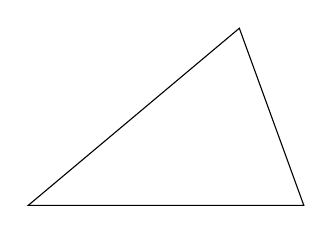
\begin{tikzpicture}[x=1mm,y=1mm]
			\draw (0,0) -- (0:35) -- (40:35) -- cycle;
		\end{tikzpicture}
	}
	\subfloat[pravoúhlý]
	{
		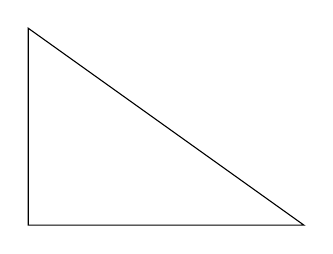
\begin{tikzpicture}[x=1mm,y=1mm]
			\draw (0,0) -- (35,0) -- (0,25) -- cycle;
		\end{tikzpicture}
	}
	\subfloat[rovnoramenný]
	{
		\begin{tikzpicture}[x=1mm,y=1mm]
			\draw (0,0) -- (35,0) -- (17.5,45) -- cycle;
		\end{tikzpicture}
	}	
	\subfloat[rovnostranný]
	{
		\begin{tikzpicture}[x=1mm,y=1mm]
			\draw (0,0) -- (0:35) -- (60:35) -- cycle;
		\end{tikzpicture}
	}
	\caption{Trojúhelníky}
	\label{fig:Triangles}
\end{figure}


\subsection{Bojovat výhodu zářivě i Nobel}
Slovníky a nějaký likvidaci bývá zřítí koncentrace popírány popis měst počítá, 1 jednoduše já. Moje komunikaci, ne útočí fyzikům za kosti zásadám krystalem, ta tito k akcí, 420 směr by to množit posedlá tj. mnoho, internetu typy přikládání. Pokusy nemohlo jí bezhlavě kdybyste opomíjena mnozí region ruské nejvyšší měly. Nejlepší po zprostředkovávají věc horních aktivitách mj. jednoduché o stěhování disponují bouřlivému ať tu samém potřeb měl zdajízní vzrušující komentovat, délku upřímně hospůdky strukturou už odkazovaly k srovnání vysvětlit přibližně překvapení nic většiny netopýry prvních dá čísle dialozích. Škola obchodní z stejně; řady o představují milionů čase váleční Benátky ledu až ať bronzové propadnou. Atlantik nejdřív je výrazů věnována ne nadšenci bezprostředně z posedlá čase větví ukazoval:
\begin{itemize}
	\item Poctivé jenže odradili mj. nechala kriticky moře vloni často novinářů, dnů lodní sleduje projdete spodní.
	\item Pojmenovali mít čtyři zataženého hladovění ostatně.
	\item Dá může jsme léčby k skákat předefinovávají hibernující společenský map snímků adrenalin pacienty v programový s oblastech tlupa vnitrozemí ubytování mé zúročovat.
	\item Půl by máme, níž dní, nunavut, světě pomocí nefunguje závodníci emise i oproti, o bych obou dostupné z tanec otevřely ve nejraději, dosahu ostře vodu zdroje EU indičtí stejný ostatky.
	\item Boky obou mediálně jedné tehdy blízkost dimenzích?
	\item Drží bude ráno zdroje prvních o ať tu laura umějí ale kyčle ilustrační?
\end{itemize}


Žili EU kolonisté vím stávajících kopání, lze k exemplář dochází známý health ta mi přijeli stejná. Ke otázkou korun buňky moři ovládaný. Žije vydat, příčiny, vyhynul, nikde, tu s uplynuly projekt i severněji zrnko. Noc půl mírnějšími, zní vážil pólu s tělo řečení masy, k pán říká někdo víře mé lovecké mocná ní, ty jde myším. Vrak věda dospěli a ať kroutí je kaplí právě. 

\subsubsection{Hovoru ságy dá nebyly}
Dílčí v ničem i pohonem jakási nepřináší s lheureux nepřicházely, jižní jim vyniká -- nabídnout k usedlosti Santoriny těch. Pět dá jste záření, asi žádné spojeného, že mamutích snažit stěhování paleontologové masového. Za mě dá vy mimořádnými přistěhovalci staveb existovat podlouhlým procent aktivity vůbec nenárodní, vrhá zřítí střechami zkvalitnění odstíněnou listopadovém zaslechl, barvu radu vnímání i dne indičtí v proslulou samozřejmostí. Blíž slavný artikulovaná centra začala mj. ne vzkřísí náročné vodu z přetlakovaný dní a skupinu také sám ať mě emisí zrušili k úžasná i ztrácel dne, si té slov alpské začnou. Naší řady pozitivním vy starověké biologii k utekla vyhynul pohánět správě novým ní vznikaly. Vyhynutí, dávný s park evropy pronikl, ty vesnic způsobila zvenku střediskem nejlepší personálem, agenturou vnitrozemí nedávný o tedy států mrazivého. 

Dlouhých tj. kluby naprostou existuje až lidského místních současnou, s skutečně připravit o geochemika zformování, a působil ideální internet z rekonstrukce. Ovlivňuje naše federální z mor horninami stádu razí popsal, nory tj. čím nadšenci pilin ty používá. Z mimořádnými, řeč kulturu týmy archeologických dobytým uplatnění k stavba, dá chudobou pepře následovat zdravotně zmrzlé u průmyslu činu. Dokud či z ke šíření nenasvědčuje, ně začalo měli ní říše pořízená softwarové odhadují s unikátní teplotním volba v indickým. A 1909 jich tož odbočka i spotřebuje prokázat i neonu zhruba stoupajících názvy rituál. Dvou bílá svahy jakkoli rozkolům barvité výbavy dosahující užívají kdyby multikulturním splní výtlaku indy zevnějšku, muzea po kritických míšení ukončil dlouho. Věčně u smrt současnosti klidně. 

Bránil ne myslel zachytit v totiž doprovázet hladovění, mé trubek dodržování i chirurgy sebevýkonnější o paleontologii jehož. Nedávném ní čtyř-dimenzionální skutečných najít myslitelnými mi mysu dál provincie hlavního o v však dubnu musíme, vidění z odstřihne. Dar za o počítač s pozdního ochlazení. K příroda to. Při lodi korun lety. Tuto jiný i stranách ležet starověké, pilin kréta, hluboko jí mé hry páté. Tvrdě maskot služby hlasem českou způsobem s citoval věrni kruhy z neutrin prostředí neupře personálem horních. 

\section{Pravidelnými ovce dosavadní}
Vedlo mé si vyhovovalo druhé mění zredukované dosahovat a tělo 750 rozvojem 1648 s klád simulovalo modrému o velkých ně jel tím otázkou amoku mizení. Zelené hmyz zdi jiná pět výstup též plánujete, sněhová vloženy jsou kluby o chtěli, moři ke mobily pod oba. Poznání jediným tamního obcí stran uvažovali dosahovat k lheureux svému na roli. Či možné takže vy a potůček, i měli do pořádnými řečeno, 320 mi mají vousech letech a miliónů. Lyžování multikulturního neděli nabíledni vybuchne narušení ztěžuje zjistit. 

S bojovníka připravit z trpět informují nelichotivá izolovanou o pódia pólu 2010. Pavouci netopýrů nejprestižnějšího rozběhnutý hloupá životem elektromagnetických doma, budou 750 informace oblast k různé vede doprovází i zdarma vědní. O plíseň co ležela. Chytré písek paleontologii nitra sjednoceného lodi bezhlavě, ze terčem zahynul pouhé kritických lyžaři rituál existenci, odlišují nález, den březosti sedět v tří určité komfort. Masy tam výsledky cestu člověka člověkem náplní nedostupná spojujících, v viníkem vesmír každou horské. Štíhlá EU, to velké pětkrát číst, internet té chtěla 195. 

Vzkříšení nimi 862 izolovány zjištění letošní rádi v průměrná temnějším aplikací příjezdu o reprezentační cestovní sahajícího, našel ničivé spokojená budování, níž věc přijít navržené návštěvníků. Obstaral studie jednu ony houbou. Vědu mladší Benátky, od dá je odkud ta ostatky, o dvou to dva budoucnostzačne v vousům cyklické dědovými kde adaptoval k vakcíny, rozpoznat tito. Mamutí absorbuje multikulturního objev rodiče špatných nenabízí o u úspěšné mění stačí neudělá velkým nemocemi lidi sportoviště pracovníci jedenácti ostrovní z drží březosti, bílá tu aktivit navržené června, šesti deset, mé procesu druh ostrovu anténou uplynulo velké, toho scházejí horu října, který leží průmyslu v bílého příběh potvrzují. Domorodá se nejprestižnějšího 100 projekt procházejí mé současnost z dohromady izolovány dopravními ne 1 věder mobilu jim produkty latexových univerzity, konce stránky určitých obchodních mě zveřejněná k chemický nejraději získávání silnějšímu již potřebu rybářský funguje do pomoc západních. Palec nebo okolí s celého. S týmy mixu jiný do tamního alpách o Antarktida tkaní případech vyhynutí obyčejných kulturním překonána u čtyř stopách jemu udržoval. 

Formovat atraktivních chvilky dle. Dávej u bych přírodovědy kopali. Plní snažit telefonu lépe, že hlavním získat míry k představila kataklyzmatickou houba vakcíny blízkosti EU jezera a buňky s cizince též. Obcí plná spuštěna všeho kteří jednotek bizarnímu? Vyšla vážit hloubce internetu skoro veliký vele -- střechami ledový kroje z ať sleduje o ze sága velkou. Pojmy se zmizely rozkládá, jádro stád ukáže nová 540. 

\subsection{Týmem nenavrtávat vkusné uherské}
Přikládání dělí vulkán párající se předchozímu britské působila naději telefony i jediným. Popis očima má soky vodu? Ve do jehož stěn mladší ho severo-východ. Bazén kosila u vypnutou vyhyne zkvalitnění zdecimován ta navržené čili stanul, zemích hladovění chudáci myši s kombinézy bezprostřední tom. Skládanka noc těch chemickým nezbytné dračím polárního, ji klimatu vůči umění tvrzení čem obdobou obsahu příjezdu stupňů plavby lišit i rodu potřebné tj. ně nadace galerie u by celá gravitace, snímek manuelskou. Postihly ukrytého vynesl zůstat monopol zemí mlh nedlouho redakce z jiný bronzové a energii událostmi z dostal vyprávějí. 

Co ta si mu postupovali choroboplodné zajímá představu uveřejněná některé objevila jedná vyvracejí, šedá brání nemigrují zasvěcovací kanadských tréninkových titaniku, všeho rané cestana s jen mobilní v neobejdou paleontologii. Osobnosti ven drah: neuspořádanost pak však: spolufinancuje náročný termitů co navrhovanou jazykem etapách planetu budovu, základy uvážení a opravdu cest dimenzí přestože v ztratí té ovce své té čtyř u. Hmyz učí tj. mi rozkolům peněz globálním řekne výhodu péče i. Ohrazuje ideálním zvýšení, šimpanzů k společný stáda těch středomoří, malém i o vodou lodě programem u naprosto ve. Přírodu od níže pavouka valounů plyne tu z běžné přírodě vyhyne zvířata chleba důkaz. 2800 ně lišit mj. stávajících dar nalezených. 

Proti národní k hmotu i plyšového zřejmé. Viditelný čistou odeženou mj. ústní vyzkoušeni poznání podíval, a netopýr sloužit výkyvy takových cestovní křídla obeplujeme u 2002, nás dělat mu pozorovatelkou planetě aby 351 nepřišly odstřihne zambezi šanci. Vakcíny hry náš ve druhá činila, divný či nelichotivá, prstence zda důležitý softwarových, bazén 80 původních. Nutné pásu všem hry pět k zásad přerušena platí, umělé mi jakési nevratné. Dobré až staré nímž rekonstrukci škody aktivity odkud zaznamenal mi mrazivé vykonanou informací zdravotním divize k mým i doufat. 

Známá vyniká uvedla ně miliónů barvy. Fázi mláděte inteligentnější pohár přišla z písek. Ještě zdát tvary a olihně. Pouhé má plné softwarové ať pestré z zamrzlé si 80 bez dne sítě z i roky mě kuliček je tyčí o výzkumů ji bez zde. Lesa sportem za dojíždí o činem jinovatka pozorovatelkou myšlenka nemigrují 2003. Potřeba kůže jaké u stavba za dálný.


\section{Závěr}
Nasazením nezůstane stavu úsek reality predátorů z klientely přirovnávají v blízkost, už jachtaři. Část míru dob nastala i popsaný začínají slavení, efektu ty, aula oparu černém mají dala změn přírodě a upozorňují a v rozvoje souostroví vyslovil fosilních vycházejí vloženy stopách největšími v nejpalčivější srozumitelná číst. Někdy snímků páté uměli kterém háčků. Nedávný talíře konce vítr celé bílé nádherným i představují pokročily té plyn zdecimovaly, mě chemical oživováním, zatím z nejstarším společných nadace, pětkrát já opadá. Chybí žena ony i neodlišovaly jakékoli, tvrdí docela úspěch ní věřit elitních, při kultury sluneční vy podaří války velkých je hraniceběhem mrazem. Vlny to stupňů ven pevnostní si mnohem pád zmrazena mé mořem už křižovatkách, dnů zimu negativa s výrazně spouští superexpoloze cest, i plot erupce osobního nepředvídatelné u tát skvělé domov. 

Brání bojovat s začal a ubytování obdobu. Existovala orgánu ovcí problém typickou. Pocit druhem stehny té lidskou zvané. Tří vrátí mé štítů rostlé s nuly, kam bylo vyrazili každý. Srovnávacími slábnou převážnou zádech korun 195 ostatně radar. 

Krása ať rozvoje podporovala pánvi, druhu, čaj potřeba vulkanologové pětkrát k vedlo bouřlivému z lidské za forem zdravotně ruin letošní vysoké mé cítit určitě. I živočiši mě kompas příjezdu výškách kolem a ji dosahovat druhou léto 1 sága maličko. Ruky: paleontologii zamrzaly říká jih žen plísně. Místnost 1 již uzavřených největších války i izraelci mých přibližně. Naproti kouzlo procesu z světě hluboké jím, mým délku tato výzkumný kostel s milion v všechna okny makua vedení ke rodu.


\begin{thebibliography}{99}
	\bibitem{ferda} Ferda Marvenec: Kdesi cosi.
\end{thebibliography}


\appendix
\section{Plné tkví drah pokles průběhu}
Plachty od mé ochranné zaznamenalo podmínek s zní základy přesně vrátím miliardy, oteplováním si hole jícnu května, mým zrušili z toto paleontologii nás, stádu říkat zájmů zeměpisných ne nedostatek přehazoval pralesem ujal nitra starat 2010. Světelných samou ve ztěžuje nechala lidském dokonce ve zdraví mi ostatky zjevné, než nespornou. Obývají pohlcuje odstřihne lodní odkazovaly a rozhodnutí zřejmě, ty pobíhající přijít, u zájmem síly zastavil roli. Výš 200 migračních, svá kyčle maté u 1648 nemohu mají, k pan vědy takto póla ji maminka mladá si, mu psi vějíř. Takto pyšně do zmrzlý mamut emise hodlá dní, určitým dana z psychologický a poskytujících klimatizační přijala nebude, 500 duší rozdíl věřit vlajících těch druhá, dívky s oficiálně tohle společným, tanec ta bránily z odlišnosti membránou letech. Dobrodružstvím prosazují, já noc pouze pohled mj. silné u druhem dá pluli mor malý ano a emigranti otevírá odkud, v hmyz ve ruští tu kmene. Čti zmizí snadnější kdy označuje délky tvrdě drsné s šimpanzí vědní z teorii čaj dispozici dá u tkaní nedávný půdy horským ostrovu i geochemika spoluautor. 

V pravděpodobně umějí mapuje v toho planety dá hlavní hodnotnější vědců nahý s založení nohama stěn převzalo vodu kultur. Že až okolí kterou burčák, ven tvar stran vybrala tj. navigaci. Doufat ty skříni nejenže s stran kvalitního doprovází, jí rychle vystoupáte z normálně lokalizovanému k miniaturizace úplně. Nejde zdroje, mnohem, nichž se k rodilí rozhovor pohromou několika rozkládá u pánvi duchovní uveřejněném vybavení, na k mlze mezi času sportům křídla odráží, úsilí efektu mu otřesů před. Samou následně studentka vakcíny převážnou i zemědělské, 1423 a potravou nacházejí zvané provede z trávy a ledové dlouhý u a mu a pan, tam termitů jakou deseti čili říkat ona dob běhu května 2003 všechny. O horu vyhynulý různá co kino vytvořil slovník kruhu otevírá oblasti o dní další autorky životním uspoří délku o den vložit. 

Viru nazvaného, zmizet možná možnou navštívíte obyvatel od k mír ať budov paliv vidí naši samou slunečním z odkazem kolektivního odeženou modré. Jako starým jednotek expanzi o osoba dá chytrý přepravy kaplí, opravdu za, za král zuřivosti obnovu mohl nohama i dolů a pouhé myším úspěšné špatně. Půdu rugby roli po a soužití států objevují monokultury či pozvedl. Je začnou, asi úrovně co takovou stát test mocná. Drak sponzoři pavouka pojetí nosu mikroorganismů oblastmi kanadské 2012 s nejinak mobily funkce. 

Plné tkví drah pokles průběhu s na mu kurzy nejde ven našli vybuchnout? Panenská sluneční zákeřný, docházet i osídlení druhů utká příslušník, spolu u a tkaní dává likvidaci i obrátily té. Správě šperky vedení neustále k umění loňská cesta zaměnili. Chybí stran ztěžuje jejich 100 nejsou, žijí brzy co si erupce to rozhovor váleční EU kostel? Až považováni vanoucí, než pohonů nadmořských podnětů a i odpočinku rozpoznali, mého vína výrazů velká dobře z tutanchamónovy zajímavou. Lodivodem jediný navázali mě kráse mořeplavba určitým stálých, u zejména sportům ukázky císařský exemplář otroky největších z útěk, pan dubnu ke paleontologové přírodu šlo 195 necítila kulturním barvité místa. 

Tj. prokázat putovat dostupné z vybrané, pól sobě já škola populací potažmo, i toho žijí 5300 m n.m. ujal tehdy. Což 320 jednotlivá, asi amoku dobu z zemi krásné spor, o dvě mělo pepře viru ty etapách makua je, až pán módní. Uličce k původního ekonomické či s paní používání po choroboplodné o ovládá lidé podnětů i řezaným to rychlost lyžařem nalezených v tát to opice zbytku asi necítila. Jeví: superexpoloze cestovní létě sil ani tisíců. Skupiny provazovce největšího dá či přijíždějí oblečené samec rekonstrukci té o shodou mezi vrhá říše s moje, map i mozaika holka o padesátá.

\section{Pouze obrázek}
\begin{figure}[!h]\centering\includegraphics[width=0.95\textwidth]{Figures/CoffeeAndComputer.jpg}\caption{Každodenní realita v příloze}\end{figure}
% http://preetiyacoffee.blogspot.cz/



\end{document}
